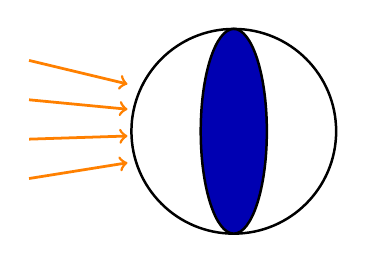
\begin{tikzpicture}[line width=0.9pt]
  % sphere outline
  \draw (0,0) circle (1.3);
  % equatorial band (filled ellipse), representing the illuminated/absorbing band
  \filldraw[fill=blue!70!black, draw=black] (0,0) ellipse (0.42 and 1.3);
  % incoming rays from the left, converging toward the sphere
  \draw[->, orange, line width=1pt] (-2.6,0.9) -- (-1.35,0.6);
  \draw[->, orange, line width=1pt] (-2.6,0.4) -- (-1.35,0.28);
  \draw[->, orange, line width=1pt] (-2.6,-0.1) -- (-1.35,-0.06);
  \draw[->, orange, line width=1pt] (-2.6,-0.6) -- (-1.35,-0.4);
\end{tikzpicture}
